\section{Materials and methods}

\subsection{Participants}

Eight naïve participants (three male, five female), aged between 22 and 29 years, gave written informed consent to participate in the study. They were all free of any known vestibular or neurological disorder and had normal or corrected-to-normal visual acuity. Participants never received any feedback about their performance. The present study was part of a larger study on the effects of eye movements on self-motion perception, some of the results of which were described in our recent report \cite{clemens2015a}. Details about the setup and methods have been described extensively in that report as well. Here we provide only a brief summary.


\subsection{Experimental setup}

Participants were seated on a motorized linear sled with their body and head restrained such that the inter-aural axis aligned with the motion axis. The sled laterally translated participants following a minimum jerk profile of fixed duration (1s) and amplitudes ranging from 1 to 27 \si{\centi\metre}. Auditory cues were suppressed using white noise presented through in-ear head-phones. Experiments were conducted in complete darkness except for visual fixation points, projected by body- or world-fixed laser pointers on a black bar, either 50 or 200 \si{\centi\metre} in front of the sled and at eye level. Eye movements were recorded at 500Hz using an EyeLink II (SR Research, Kanata, Canada) system. Eye position was calibrated before each session using 11 evenly spaced calibration points ranging from -22 to 22 degrees.


\subsection{Paradigm}

We used a two-alternative forced choice (2-AFC) task to study the influence of fixation depth on the perception of linear translation. We tested two fixation depths: near (50 cm) and far (200 \si{\centi\metre}) and two different eye fixation conditions: world-, and body-fixed fixation. A trial contained two sequential motion intervals of equal duration (1s), with the motion in the same direction (either leftward or rightward). Fixation condition (world, or body-fixed) was the same in both intervals, but a different fixation depth was presented in each. Participants had to judge whether the translation during the second motion interval was longer or shorter than in the first motion interval.

\begin{figure}
    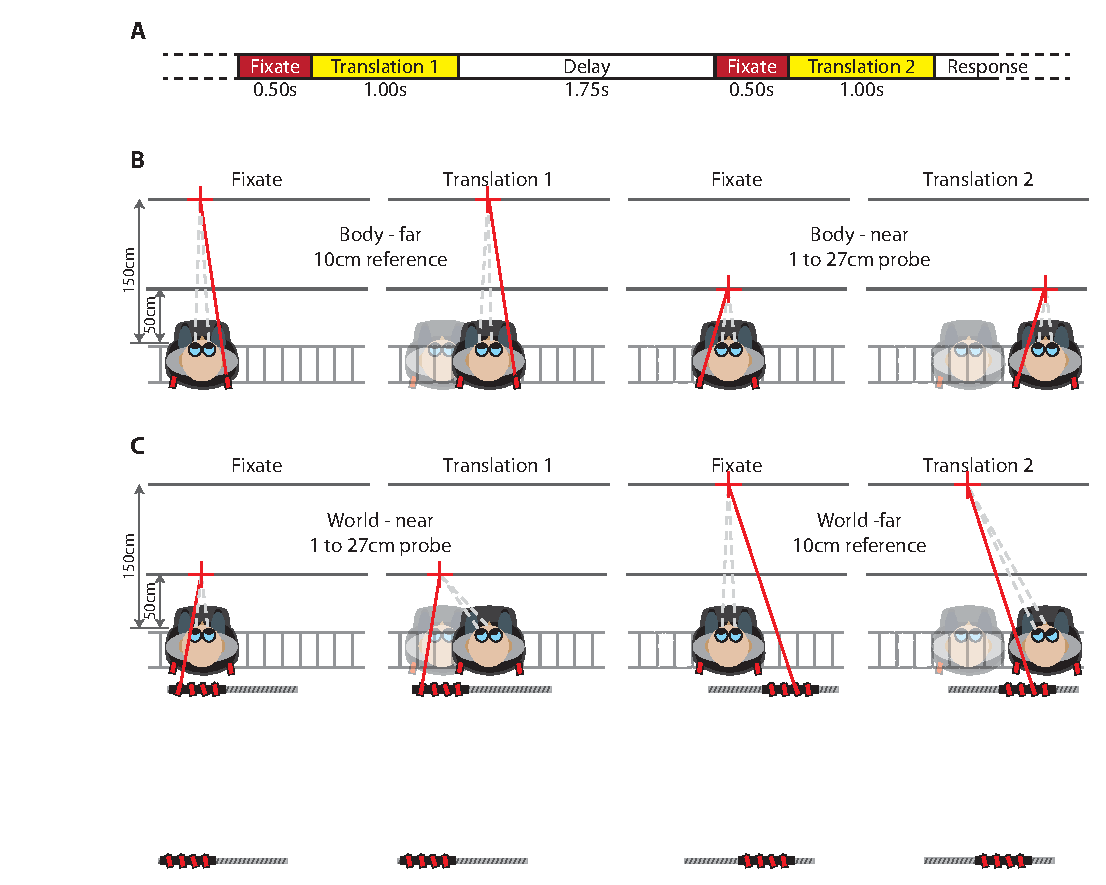
\includegraphics[width=1.0\textwidth]{src/paper4/paper4_figure1.eps}

    \caption{...}
    \label{p4:fig1}    
\end{figure}
 
The timing of a single trial is shown in \figref{p4:fig1}A. Each trial started with the onset of a central fixation point (i.e. aligned between the eyes) for 0.5s. Subsequently, the first 1s motion interval commenced, during which the fixation type which was at on the the two depths, remained stationary (world) or moved along with the participant (body). Subsequently a 1.75s delay followed in which the participant was kept in complete darkness. Then, the central fixation point reappeared, followed 0.5s later by a second 1s translation interval, with the same fixation condition but with fixation point at the other depth as in the first interval. Finally, the participant responded by moving a 1-dimensional joystick away from (longer) or towards (shorter) the body. Top-view illustrations of body-centered and world-centered trials are shown in Figures 1B and 1C respectively.

\begin{table}
    \begin{tabular}{llll}
    Comparison & Reference & 1st interval & Direction \\
    \hline
    Body & Near & Reference & Right \\
    Near vs. far & & & Left \\    
    & & Probe & Right \\
    & & & Left \\
    \cline{2-4}
	& Far & Reference & Right \\
    & & & Left \\    
    & & Probe & Right \\
    & & & Left \\
    \hline
    World & Near & Reference & Right \\
    Near vs. far & & & Left \\    
    & & Probe & Right \\
    & & & Left \\
    \cline{2-4}
	& Far & Reference & Right \\
    & & & Left \\    
    & & Probe & Right \\
    & & & Left \\
    \end{tabular}

    \caption{List of the 2 main comparisons that we tested. The (10cm) reference movement was presented in either the first or the second interval. We also manipulated movement direction (leftward vs rightward) yielding a total of 16 trial types.}

    \label{p4:tab1}
\end{table}

Across trials, we varied fixation distance, as well as the order of reference and probe, giving a total of four variations per condition (see \tabref{p4:tab1}). Movement direction (either leftward or rightward) alternated between consecutive trials. The size of the probe translation was adaptively chosen based on the participants' earlier responses (Psi method; {Kontsevich:1999tg}) to determine the point of subjective equality. This was done separately for all 16 trial types (2 main conditions x 2 reference stimuli x 2 reference/probe orders x 2 movement directions; see Table 1). A total of 25 trials were collected per trial type yielding a total of 200 trials for each of the two main conditions.

Trials were presented in two one-hour sessions. To prevent dark adaptation, we turned on the lights for 5s after each block of 8 trials, and for at least 30 s after every 2 blocks. Each of the 16 unique trial types were presented once every 2 blocks. After each block, the adaptive procedure determined which translation size to test in the following block. To increase the number of data-points available to the adaptive psychometric procedure at the beginning of the experiment, we collapsed across movement direction and reference order for the first 10 trials. After that, the procedure ran separately for each of the 16 distinct trial types.

\subsection{Data analysis}

For each combination of the two main conditions and the two reference/probe orders (see \tabref{p4:tab1}), we quantified the perceived probe translation by calculating the probability the probe translaton was pereived longer than the reference translation as a function of actual probe translation. We used a maximum likelihood fit of a cumulative Gaussian function to summarize the psychometric data:

\begin{equation}
\label{p4:eq1}
P(x) = \lambda + (1 - 2\lambda) \frac{1}{\sigma \sqrt{2\pi}} \int_{-\infty}^{x}{e^{-(y-\mu)^2 / 2\sigma^2}}dy,
\end{equation}

in which $|x|$ represents the size of the probe translation. The mean of the Gaussian, PSE, represents the point of subjective equality. The slope of the curve reflects the precision ($1/\sigma$) of reference-probe discrimination performance. Parameter $\lambda$, representing the lapse rate, accounts for stimulus-independent errors caused by subject lapses or mistakes and was restricted to small values ($\lambda < 0.06$). Fits were performed using the Psignifit toolbox {Wichmann:2001ud, Wichmann:2001wa}.
For each trial type (see \tabref{p4:tab1}), we also quantified eye movements, corrected for drift based on initial fixation. We discarded trials containing blinks as well as trials where the final eye position was more than two standard deviations away from the condition average. In total, about 12\% of all trials were discarded. After rejecting trials, we computed the average ratio between the actual, , and ideal eye movement angle that would have occured in the world-fixed fixation condition (Equation 2). This ideal eye movement angle is computed by taking the arc-tangent of the actual translation distance, , divided by the fixation depth, . We computed this ratio, , for every condition c (see Table 1). Note that for body fixation the normalized eye movement would be  and for world fixation would be .

\begin{equation}
\label{p4:eq2}
\end{equation}

Using this ratio, , we can compute the expected eye movement,  at arbitrary translation distances, even ones we did not explicitly measure:

\begin{equation}
\label{p4:eq3}
\end{equation}

Model
Using the simple cue integration model we introduced in our previous paper (Clemens et al., 2014) as a starting point, we investigate the manner in which fixation depth is taken into account. As in our previous paper, we model the perceived distance, , as a weighted combination of a vestibular, , and oculomotor estimate of translation,  (Equation 4). 

\begin{equation}
\label{p4:eq4}
p_i = \alpha_{d_i} \hat{\varphi}_i + (1 - \alpha_{d_i}) m_i
\end{equation}

As the weighting parameter, , can depend on fixation depth,, it can explain both fixation depth depedent as well as independent effects. The exact distribution between these components can be found by analyzing the weighting parameter. If the weighting parameter is the same across all values for fixation depth , then there is no depth dependent part. Similarly, highly different parameters would indicate depth dependent effect. Further note that while we assume that that the vestibular () and oculomotor weights ( sum to one, they could sum to any arbitrary value by scaling the weights appropriately. 
By definition, the probe displacement (subscript p) is perceived as equal in length to the 10 cm reference displacement (subscript r) at the PSE, . By substituting both sides by the right hand side of Equation 4, we obtain:

\begin{equation}
\label{p4:eq5}
\alpha_{d_r} \hat{\varphi}_i + (1 - \alpha_{d_r}) m_i = \alpha_{d_p} \hat{\varphi}_i + (1 - \alpha_{d_p}) m_i + \epsilon
\end{equation}

In the present experiment, the reference displacement, , was always 10 cm and the probe displacement, , was equal to the measured PSE for the presented combination of fixation types (i.e,  in Equation 1). This model (i.e. Equation 5) was then fit to data from the body and world conditions using linear regression, finding one weight for every fixation depth (that is,  and ) that minimizes the sum of squared errors (. 
As mentioned before, these weights model both depth dependent as well as depth independent effects. Perfect compensation for fixation depth would require multiplication of the eye movement angle by the actual fixation depth, . The actual value of  used depends on the relative amount of compensation for fixation depth. This means that   and, in the specific case of our near and far targets,  and . By dividing our parameters, we remove the depth independent part  and reveal the ratio of fixation depth value used for compensation, . In case of perfect compensation the expected ratio is be , while in case of no compensation it is 1.
